Please find a research problem in your area that requires optimizaiton
techniques to solve the problem. For this problem, you need to explain
the problem and formulate it as an optimization problem. Then you need
to discuss how this problem is solved.

\textbf{Note:} The problem does not have to be convex and you may
use other techniques beyond this course.\\

For the question for part 2, I decided to consider one of the application problems
from the additional excercises for our textbook.  The problem is 15.6 and is stated
as follows:\\

\textbf{Maximizing Algebraic Connectivity of a Graph}\\

Let $G = (V, E)$ be a weighted undirected graph with $n = \vert V \vert$ nodes,
$m = \vert E \vert$ edges, and weights $w_{1}, \ldots, w_{m} \in \mathbf{R_{+}}$ on
the edges. If edge $k$ connects nodes $i$ and $j$, then define $a_{k} \in \mathbf{R^{n}}$
as $(a_{k})_{i} = 1, (a_{k})_{j} = -1$, with other entries zero.  The weighted Laplacian
(matrix) of the graph is defined as
\[
L = \sum_{k = 1}^{m} w_{k} a_{k} a_{k}^{T} = A \mbox{\textbf{diag}}(w)A^{T}
\]
where $A = [ a_{1} \ldots a_{m} ] \in \mathbf{R^{n \times m}}$ is the incidence matrix of the
graph. Nonnegativity of the weights implies $L \succeq 0$.

Denote the eigenvalues of the Laplacian $L$ as
\[
\lambda_{1} \leq \lambda_{2} \leq \cdots \leq \lambda_{n}
\]
which are functions of w. The minimum eigenvalue $\lambda_{1}$ is always zero, while the second smallest
eigenvalue $\lambda_{2}$ is called the algebraic connectivity of $G$ and is a measure of the connectedness of
a graph: The larger $\lambda_{2}$ is, the better connected the graph is. It is often used, for example, in
analyzing the robustness of computer networks.

Though not relevant for the rest of the problem, we mention a few other examples of how the
algebraic connectivity can be used. These results, which relate graph-theoretic properties of $G$
to properties of the spectrum of $L$, belong to a field called spectral graph theory. For example,
$\lambda_{2} > 0$ if and only if the graph is connected. The eigenvector $\nu_{2}$ associated with$\lambda_{2}$ is often called
the Fiedler vector and is widely used in a graph partitioning technique called spectral partitioning,
which assigns nodes to one of two groups based on the sign of the relevant component in $\nu_{2}$ . Finally,
$\lambda_{2}$ is also closely related to a quantity called the isoperimetric number or Cheeger constant of $G$,
which measures the degree to which a graph has a bottleneck.

The problem is to choose the edge weights $w \in \mathbf{R^{m}_{+}}$ , subject to some linear inequalities (and the
nonnegativity constraint) so as to maximize the algebraic connectivity:
\begin{eqnarray*}
\mbox{minimize} & \lambda_{2}\\
\mbox{subject to} & w \succeq 0, Fw \preceq g
\end{eqnarray*}
with variable $w \in \mathbf{R^{m}}$ . The problem data are $A$ (which gives the graph topology), and $F$ and $g$
(which describe the constraints on the weights).
\begin{enumerate}[(a)]
\item{Describe how to solve this problem using convex optimization.

Here we are going to first make sure that $\lambda_{2}$ is a concave function of $w$. So, we will need to construct a matrix so that the smallest eigenvalue is $\lambda_{2}$, since this will help use make sure that $\lambda_{2}$ is concave.

Now, we will note that $\mathbf{1}$ is an eigenvector of $L$. Now, if we were to restrict our space to $\mathbf{1}^{\perp}$, then we can express $\lambda_{2} = \lambda_{min}(Q^{T}LQ)$, where $Q \in \mathbf{R^{n \times (n-1)}}$.  Now, $Q$ is therefore a matrix whose columns for an orthogonal basis for $N(\mathbf{1}) = \mathbf{1^{\perp}}$, so that $Q^{T}LQ$ has eigenvalues $\lambda_{2}(L),\ldots,\lambda_{n}(L)$.  So, our problem is now
\begin{eqnarray*}
\mbox{maximize} & \lambda_{min}(Q^{T}LQ)\\
\mbox{subject to} & w \succeq, \quad Fw \preceq g
\end{eqnarray*}}

\item{Numerical example. Solve the problem instance given in max\_alg\_conn\_data.m, which uses
$F = \mathbf{1}^{T}$ and $g = 1$ (so the problem is to allocate a total weight of 1 to the edges of the graph).
Compare the algebraic connectivity for the graph obtained with the optimal weights $w^{*}$ to the
one obtained with $w^{unif} = (1/m)\mathbf{1}$ (i.e., a uniform allocation of weight to the edges).
Use the function plotgraph(A,xy,w) to visualize the weighted graphs, with weight vectors
$w^{*}$ and $w^{unif}$ . You will find that the optimal weight vector $v^{*}$ has some zero entries (which
due to the finite precision of the solver, will appear as small weight values); you may want to
round small values (say, those under 10 −4 ) of $w^{*}$ to exactly zero. Use the gplot function to
visualize the original (given) graph, and the subgraph associated with nonzero weights in $w^{*}$.
Briefly comment on the following (incorrect) intuition: “The more edges a graph has, the more
connected it is, so the optimal weight assignment should make use of all available edges.”
\begin{figure}[h!]
  \centering
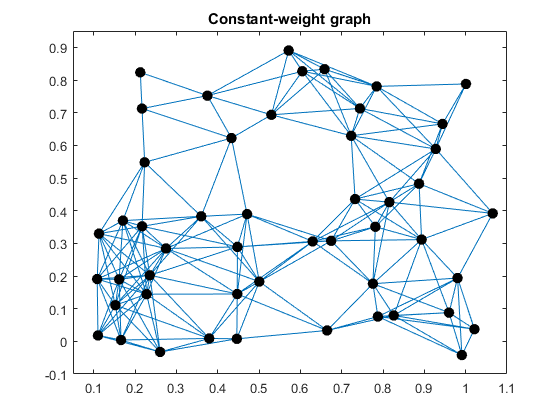
\includegraphics[width=\textwidth]{source/part2/fig1}
%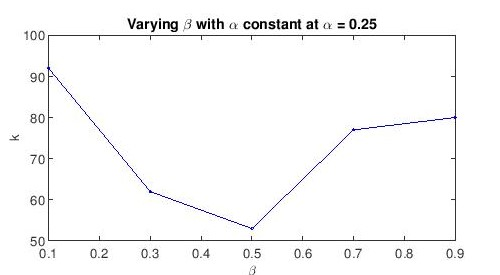
\includegraphics[width=5cm]{source/prob1/fig4}
\caption{Comparison of the convergence of Backtracking line search with varying $\alpha$ and $\beta$}
\end{figure}
\begin{figure}[h!]
  \centering
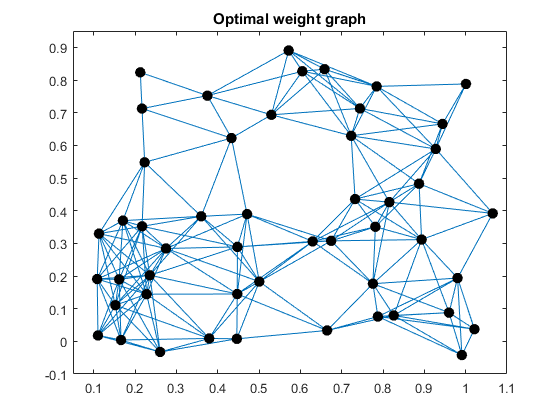
\includegraphics[width=\textwidth]{source/part2/fig2}
%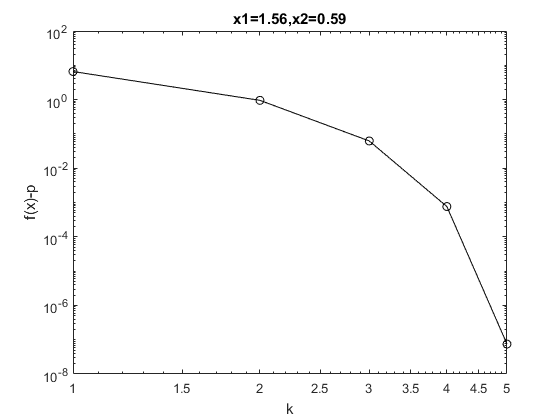
\includegraphics[width=5cm]{source/part2/fig4}
\caption{Comparison of the convergence of Backtracking line search with varying $\alpha$ and $\beta$}
\end{figure}}
\end{enumerate}